%%%%%%%%%%%%%%%%%%%%%%%%%%%%%%%%%%%%%%%%%%%%%%%%%%%%%%%%%%%%%%%%%%%%%%%%%%%%%%%%%%%%%%%%%%%%%%%%%%%%
% Project Requirements Specification Report
% Authors: Michael Galliers and James Miller
% Course: CSC 440
%%%%%%%%%%%%%%%%%%%%%%%%%%%%%%%%%%%%%%%%%%%%%%%%%%%%%%%%%%%%%%%%%%%%%%%%%%%%%%%%%%%%%%%%%%%%%%%%%%%%

\documentclass[12pt]{article}
\usepackage[utf8]{inputenc}
\usepackage{graphicx}
\usepackage{float}
\usepackage{tocloft}
\usepackage{array}
\usepackage[]{algorithm2e}
\usepackage[T1]{fontenc}
% Page margins
\usepackage[letterpaper, portrait, margin=1in]{geometry}

% Document configuration

% Section numbering
\renewcommand \thesection{\Roman{section}}
\renewcommand \thesubsection{\Alph{subsection}.}

% Environment config for requirements
%  - Configures formatting of the section heading and numbered, nested lists
\newenvironment{requirement}[1]
{
    % Format requirement sections (R1. ...)
    \renewcommand{\thesubsubsection}{R\arabic{subsubsection}.}
    % Format nested, numbered lists (1.1, 1.1.1, 1.1.1.1, ...)
    \renewcommand{\labelenumi}{
        \arabic{subsubsection}.\arabic{enumi}
    }
    \renewcommand{\labelenumii}{
        \arabic{subsubsection}.\arabic{enumi}.\arabic{enumii}
    }
    \renewcommand{\labelenumiii}{
        \arabic{subsubsection}.\arabic{enumi}.\arabic{enumii}.\arabic{enumiii}
    }
    \renewcommand{\labelenumiv}{
        \arabic{subsubsection}.\arabic{enumi}.\arabic{enumii}.\arabic{enumiii}.\arabic{enumiv}
    }
    % Create the subsubsection for the requirement
    \subsubsection{#1}
    \begin{enumerate}
}
{
    \end{enumerate}
}

% Dictionary table environment
\newenvironment{dictionary}[1]
{
    \subsection{#1}
    \begin{table}[H]
    \begin{tabular}{ | m{\dimexpr.45\linewidth-1\tabcolsep-1.3333\arrayrulewidth}
                     | m{\dimexpr.55\linewidth-1\tabcolsep-1.3333\arrayrulewidth} | }
    \hline
    \textbf{Term} & \textbf{Description} \\ \hline
}
{
    \end{tabular}
    \end{table}
}

% How to format a row in the dictionary
\newcommand{\dictitem}[2]{\detokenize{#1} & #2 \\ \hline}

% Set path to all graphics
\graphicspath{{figures/}{build/diagrams/}}

% Do paragraph indenting after section tags
\usepackage{indentfirst}

% Adjust space between numbers and headings in table of contents
\addtolength{\cftsecnumwidth}{12pt}
\addtolength{\cftsubsubsecnumwidth}{-10pt}


\author{Michael Galliers}
\title{CSC 440 - Requirements Specification Report}


\begin{document}

\begin{titlepage}
\maketitle
\end{titlepage}

\newpage
    \tableofcontents
\newpage

% No styling
\thispagestyle{empty}
% Include a table of figures
\listoffigures
% New page
\newpage

\section{Introduction}
\subsection{Problem Statement}
As EKU college students, we the authors have firsthand experience with the difficulties of
grade/progress management. The tools already used by the college for grade management have their
flaws. Many professors either do not setup the grading categories and weights properly, or they
choose to not use BlackBoard for tracking grades at all. Also, BlackBoard does not have the ability
to give advanced insights for student grades other than simple weighted averages or totals.

Students can choose to manage their grades on their own, either using technology, such as
spreadsheets, or pen and paper. Students who do this are able to gain more insights into their
progress in courses, but it can be very time consuming to setup spreadsheets or do computations by
hand, especially when predicting grades needed on an assignment.

\subsection{Proposal}
As a solution to these problems, we propose a software system for grade and progress tracking. The
system shall have 2 main related components: one for grade tracking and one for major/concentration
progress tracking. The grade tracking system will allow students to easily enter and track their
grades across colleges, semesters, courses, and categories (homework, exams, etc.). Various views on
the user interface will display grades/scores using visual elements and animations, making it easy
for students to see how well they are doing.

The second component of the application is a progress tracker for majors and concentrations.
Information provided through the grade tracking feature, coupled with course requirements structures
will allow students to view their progress across multiple majors and concentrations.

\section{System Description}
The system shall have a user account management component to keep track of students, including the
ability to register, login, edit account, and logout. When a student logs into the system, the
student shall see a dashboard containing the most relevant information and navigation links. From
there, the student will also be able to access the system menu, allowing them to navigate to either
the grade tracking component or the progress tracking component.

\subsection{Grade Tracking Component}
\noindent
The grade tracking component shall have views for the following items:

\begin{enumerate}
    \item All semesters (root grade tracking view)
    \item Courses in a semester
    \item Details of a course (including categories and grade entries)
\end{enumerate}

The \textit{All Semesters} view shall allow the student to navigate to a particular semester,
add/remove a semester in which they are enrolled, and view statistics about his/her grades in that
semester.

The \textit{Courses} view shall display the courses that are in a particular semester. The student
shall be able to add/remove/edit courses, view statistics for grades in each course, and navigate
to any of the courses.

The \textit{Course Detail} view shall display all remaining details for a particular course. This
includes the statistics of a student's grades in the course, the grading categories of the course,
and the grade entries themselves. The student shall also have the ability to add/remove/edit
categories and grade entries.

\subsection{Progress Tracking Component}
\noindent
The progress tracking component shall allow students to track their progress across major
concentrations. This component shall have the following hierarchical views:

\begin{enumerate}
    \item Colleges (root progress tracking view)
    \item Majors
    \item Concentrations
    \item Concentration progress
\end{enumerate}

The \textit{Colleges} view shall display the colleges in which the student is enrolled and allow
him/her to navigate to the \textit{Majors} view for that college. The student shall also have the
ability to add/remove colleges which he/she is enrolled in.

The \textit{Majors} view shall display the majors of the college which was navigated from that the
student is enrolled in. The student shall be able to add/remove majors which he/she is enrolled in
and also navigate to the \textit{Concentrations} view for a particular major.

The \textit{Concentrations} view shall display \textbf{all} the concentrations of the major which
was navigated from, broken up into 2 sections: one for the concentration(s) the student in enrolled
in and one for all other concentrations. The student shall be able to add/remove concentrations
which they are enrolled in and navigate to the \textit{Concentration progress} view.

The \textit{Concentration progress} view shall display visuals for the student's progress in the
concentration, including overall progress and individual courses completed. This view shall be based
on courses the student has entered through the grade tracking component.

\section{System Requirements}
\subsection{Functional Requirements}

% Some common text/sequences that are used a lot...
\newcommand{\sysshall}{The system shall }
\newcommand{\stushall}{The student shall }
\newcommand{\usershall}{The user shall }
\newcommand{\loginpage}{\sysshall display the login page.}
\newcommand{\mainmenu}{\sysshall display the main menu.}
\newcommand{\clickmainmenu}{\stushall click the \textbf{Main Menu} button}
\newcommand{\redirecthome}{\sysshall redirect the student to the homepage.}
\newcommand{\gotohome}{
    \item \clickmainmenu
    \item \mainmenu
}

\begin{requirement}{\sysshall allow a user to register for an account}
    \item \loginpage
    \item \usershall click the \textbf{Register} button.
    \item \sysshall display the \emph{Registration} page.
    \item \usershall enter the requested information.
    \item \usershall click the \textbf{Register} button.
    \item \sysshall validate the information entered by the user.
    \begin{enumerate}
        \item If the entered information is invalid, the system shall display warnings next to the
        relevant fields.
    \end{enumerate}
    \item \redirecthome
\end{requirement}

\begin{requirement}{\sysshall allow a student to login to his/her account}
    \item \loginpage
    \item \stushall enter his/her login credentials.
    \item \sysshall validate the credentials.
    \begin{enumerate}
        \item If the credentials are not valid, the system shall display warnings next to the
        fields with errors.
    \end{enumerate}
    \item \redirecthome
\end{requirement}

\begin{requirement}{\sysshall allow a student to logout of his/her account}
    \item \mainmenu
    \item \stushall click the \textbf{Logout} button.
    \item \loginpage
\end{requirement}

\begin{requirement}{\sysshall allow a student to view progress in a concentration}
    \item \mainmenu
    \item \stushall click the \textbf{Concentration Progress} button.
    \item \sysshall display the \emph{Concentration Progress} page.
    \item \stushall select the college which the concentration is in.
    \item \stushall select the major which the concentration is in.
    \item \stushall select the concentration.
    \item \stushall click the \textbf{Load Progress} button.
    \item \sysshall display the concentration requirement structure.
    \gotohome
\end{requirement}

% Shortcut for navigating to semester page
\newcommand{\navsemesters}{
    \item \mainmenu
    \item \stushall click the \textbf{Semesters} button.
    \item \sysshall display the semesters the student is enrolled in.
}

\begin{requirement}{\sysshall allow a student to view enrolled semesters}
    \navsemesters
    \gotohome
\end{requirement}

\begin{requirement}{\sysshall allow a student to add/remove enrolled semesters}
    \navsemesters
    \item \stushall click the \textbf{Add Semester} button.
    \item \sysshall display the \emph{Add Semester} form.
    \item \stushall select the semester to add.
    \item \stushall click the \textbf{Save} button.
    \item \sysshall add that semester to the semesters shown.
    \item \stushall click the \textbf{Delete} button next to one of the semesters.
    \item \sysshall display a delete confirmation message.
    \item \stushall click the \textbf{Yes, Delete} button.
    \item \sysshall remove that semester from the semesters shown.
    \gotohome
\end{requirement}

% Shortcut for navigating to enrolled courses
\newcommand{\navcourses}{
    \navsemesters
    \item \stushall click the chosen semester.
    \item \sysshall display the courses the student is enrolled in, in the selected semester.
}

\begin{requirement}{\sysshall allow a student to view enrolled courses}
    \navcourses
    \gotohome
\end{requirement}

\begin{requirement}{\sysshall allow a student to add/remove enrolled courses}
    \navcourses
    \item \stushall click the \textbf{Add Course} button.
    \item \sysshall display the \emph{Add Course} form.
    \item \stushall select the course to add.
    \item \stushall click the \textbf{Save} button.
    \item \sysshall add that course to the courses shown.
    \item \stushall click the \textbf{Delete} button next to one of the courses.
    \item \sysshall display a delete confirmation message.
    \item \stushall click the \textbf{Yes, Delete} button.
    \item \sysshall remove that course from the courses shown.
    \gotohome
\end{requirement}

% Shortcut for navigating to course details
\newcommand{\navcoursedetails}{
    \navcourses
    \item \stushall click the chosen course.
    \item \sysshall display the course details for the selected course.
}

\begin{requirement}{\sysshall allow a student to view course details}
    \navcoursedetails
    \gotohome
\end{requirement}

\begin{requirement}{\sysshall allow a student to add/edit/remove grade entries}
    \navcoursedetails
    \item \stushall click the \textbf{Add Grade Entry} button under one of the categories.
    \item \sysshall display the \emph{Grade Entry} form.
    \item \stushall enter the information required.
    \item \stushall click the \textbf{Save} button.
    \begin{enumerate}
        \item If any of the fields are invalid, the system shall display warnings next to those
        fields which are invalid.
    \end{enumerate}
    \item \sysshall add the new grade entry to the grade entries shown.
    \item \stushall click the \textbf{Edit} button next to one of the grade entries.
    \item \sysshall display the \emph{Grade Entry} form, populated with the selected grade entry's
    information.
    \item \stushall edit the grade entry information.
    \item \stushall click the \textbf{Save} button.
    \begin{enumerate}
        \item If any of the fields are invalid, the system shall display warnings next to those
        fields which are invalid.
    \end{enumerate}
    \item \sysshall update the grade entry information on the course details page accordingly.
    \item \stushall click the \textbf{Edit} button next to one of the courses.
    \item \sysshall display the \emph{Grade Entry} form, populated with the selected grade entry's
    information.
    \item \stushall click the \textbf{Delete} button.
    \item \sysshall display a delete confirmation message.
    \item \stushall click the \textbf{Yes, Delete} button.
    \item \sysshall remove that grade entry from the course details page.
    \gotohome
\end{requirement}

% \subsection{Non-functional Requirements}

% \subsection{Domain Requirements}

\begin{figure}[p!]
  \section{Use-case Diagram}
  \centering
  \includegraphics[width=0.8\linewidth]{use_case_diagram.pdf}
  \caption{Use-case Diagram}
\end{figure}

\begin{figure}[p!]
  \section{Data Flow Diagrams}
  \subsection{Level 0 DFD}
  \centering
  \includegraphics[width=\linewidth]{level_0_dfd.pdf}
  \caption{Level 0 DFD}
  \begin{flushleft}
    The system frontend passes user account information to the API to register for, login and logout
    of user accounts. The frontend communicates with the backend API by use of data object IDs to
    perform various tasks. Grade entries can be created and passed to the API as data structures.
    The API gives the frontend access to all the main data structures so they can be used for
    calculations and rendering.
  \end{flushleft}
\end{figure}

\begin{figure}[p!]
  \subsection{Level 1 DFD}
  \centering
  \includegraphics[width=\linewidth]{level_1_dfd.pdf}
  \caption{Level 1 DFD}
  \begin{flushleft}
    The level one DFD depicts the main use cases of the backend API. All but one of the main use
    cases is generic enough that the implementation is not worth decomposing further (already
    implemented by software libraries). In these use cases, the word \emph{manage} is referring to
    being able to create, retrieve, update and delete the data structure. The \emph{Calculate
    Concentration Progress} process is for constructing a recursive data structure representing the
    requirement structure of a concentration, including which requirements/courses the student has
    completed.
  \end{flushleft}
\end{figure}

\begin{figure}[p!]
  \subsection{Level 2 DFD: P4}
  \centering
  \includegraphics[width=\linewidth]{level_2_dfd_p4.pdf}
  \caption{Level 2 DFD: P4}
  \begin{flushleft}
    \emph{Authenticate Student} verifies that the student is authenticated by checking their auth
    token. The \emph{Retrieve Requirement} process uses the collge, major and concentration IDs to
    narrow down which concentration is in question and get the root requirement for that
    concentration. \emph{Generate Requirement Structure} works in a recursive manner with 
    \emph{Check Fulfillment} to generate the requirements structure for a particular concentration's
    root requirement, checking whether the requirement is fulfilled at each level.
  \end{flushleft}
\end{figure}

\begin{figure}[p!]
  \subsection{Level 3 DFD: P4.4}
  \centering
  \includegraphics[width=\linewidth]{level_3_dfd_p4-4.pdf}
  \caption{Level 3 DFD: P4.4}
  \begin{flushleft}
    \emph{Check Course Requirements} checks whether the minimum number of directly related courses
    have been completed. \emph{Check Sub-Requirements} checks if the minimum number of
    sub-requirements have been fulfilled. \emph{Check Sub-Requirement Course Count} checks if at
    least the minimum number of courses in directly related sub-requirements have been completed.
    The \emph{Check Fulfilled} process then uses the outputs of the previous three processes to
    determine if the requirement has been fulfilled.
  \end{flushleft}
\end{figure}

\clearpage

\begin{figure}[p!]
  \section{Structure Chart}
  \centering
  \includegraphics[width=0.8\linewidth]{top_level_structure_chart.pdf}
  \caption{Structure Chart}
  \begin{flushleft}
    The \emph{Top Decider} represents the server software running the API; requests to particular
    URLs are matched to the actions just beneath it. As mentioned in the DFD diagrams, all but one
    of the first level functions are not expanded further, since the functionality is generic enough
    for software libraries to handle the requests with little modification. The \emph{Calculate
    Concentration Progress} function first checks that the student is authenticated before
    subsequently retrieving the concentration's root requirement and generating the requirement
    structure. In order to generate the requirement structure, the fulfillment of the three main
    requirements must be checked, as mentioned in the DFD section. If any of the conditions are not
    fulfilled, subsequent conditions are not checked.
  \end{flushleft}
\end{figure}

% \section{Activity Diagrams}

\begin{figure}[p!]
  \section{Database Design}
  \subsection{ER Schema}
  \centering
  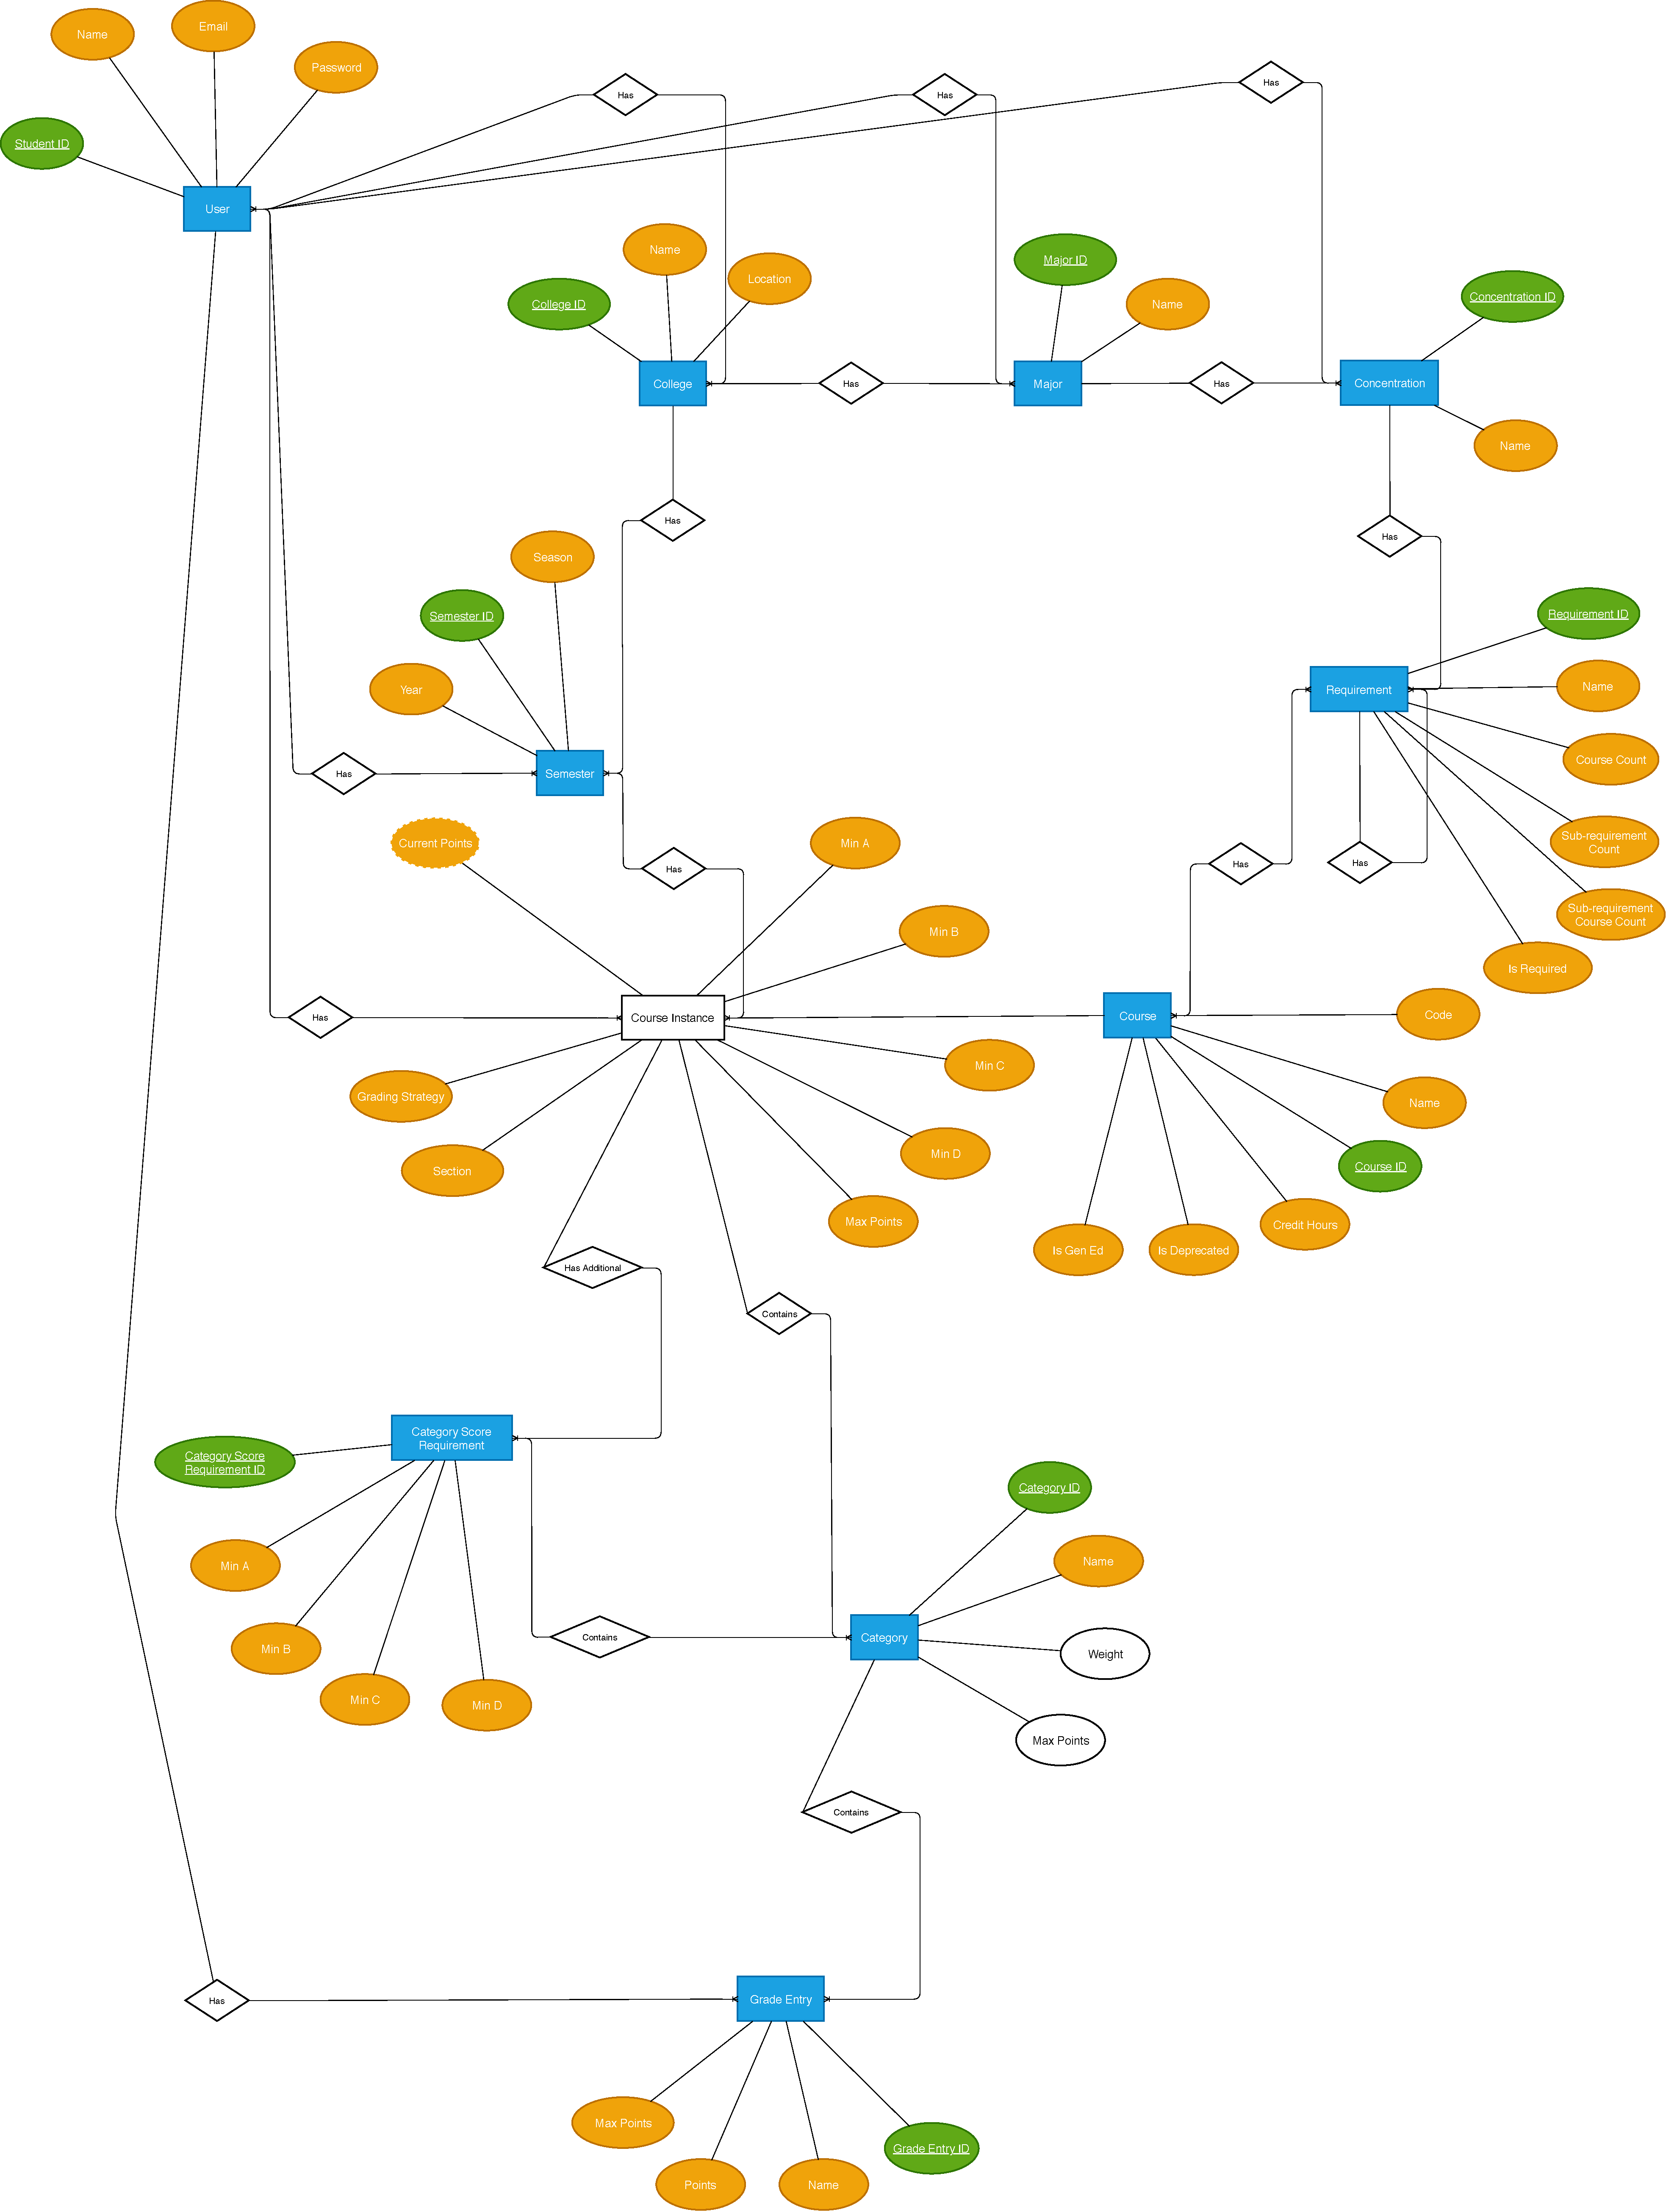
\includegraphics[width=0.85\linewidth]{database_erd.pdf}
  \caption{Database ERD}
  \begin{flushleft}
    The database diagram depicts the entities and relationships that will make up the database.
    \textbf{Note}: The \emph{Table Schema} section was omitted, since table creation is handled by
    the Django ORM.
  \end{flushleft}
\end{figure}

\clearpage

% \subsection{Table Schema}

\section{Algorithm Design}
% Python formatting for pseudo code
\newcommand{\forcond}{$i=0$ \KwTo $n$}
\SetStartEndCondition{ }{}{}%
\SetKwProg{Fn}{def}{\string:}{}
\SetKwFunction{Range}{range}%%
\SetKw{KwTo}{in}
\SetKw{KwIn}{in}
\SetKw{KwIs}{is}
\SetKwFor{For}{for}{\string:}{}%
\SetKwIF{If}{ElseIf}{Else}{if}{:}{elif}{else:}{}% \SetKwFor{While}{while}{:}{fintq}%
\renewcommand{\forcond}{$i$ \KwTo\Range{$n$}} \AlgoDontDisplayBlockMarkers\SetAlgoNoEnd\SetAlgoNoLine%

\subsection{Check Course Requirements}
\begin{algorithm}[H]
\SetKwFunction{CourseRequirementsFulfilled}{are\_course\_requirements\_fulfilled}%
\Fn{\CourseRequirementsFulfilled{student, course\_count, courses}}{
  \KwData{Student whose requirement fulfillment is being checked, minimum number of completed
  courses required to fulfill the requirement, the courses in this requirement}
  \KwResult{Whether the course requirements are fulfilled for the student}
  \tcc{If no course count requirement, it is fulfilled by convention}
  \If{course\_count \KwIs None}
  {
    \Return{true}
  }
  $count = 0$\\
  \For{$course$ \KwTo $courses$}{
    \If{is\_fulfilled(student, course)}
    {
      $count += 1$\\
    }
  }
  \tcc{Assert that the number of courses completed is greater than or equal to the minimum required}
  \Return{$count \geq course\_count$}
}
\end{algorithm}

\subsection{Check Sub-Requirements}
\begin{algorithm}[H]
\newcommand{\SubReqCnt}{sub\_requirement\_count}
\newcommand{\SubReqs}{sub\_requirements}
\newcommand{\SubReq}{sub\_requirement}
\newcommand{\student}{student}


\SetKwFunction{SubRequirementsFulfilled}{are\_sub\_requirements\_fulfilled}%
\Fn{\SubRequirementsFulfilled{\student, \SubReqCnt, \SubReqs}}{
  \KwData{Student whose requirement fulfillment is being checked, minimum number of sub-requirements
  required to fulfill the requirement, the sub-requirements of this requirement}
  \KwResult{Whether the minimum number of sub requirements are fulfilled for the student}
  \tcc{If no minimum sub-requirement count requirement, it is fulfilled by convention}
  \If{$\SubReqCnt$ \KwIs $None$}
  {
    \Return{$true$}
  }
  $count = 0$\\
  \For{$\SubReq$ \KwIn $\SubReqs$}{
    \If{is\_fulfilled($\student$, $\SubReq$)}
    {
      $count += 1$\\
    }
  }
  \tcc{Assert that the number of sub-requirements completed is greater than or equal to the minimum
  required}
  \Return{$count \geq \SubReqCnt$}
}
\end{algorithm}

\subsection{Check Sub-Requirement Course Count}
\begin{algorithm}[H]
\newcommand{\SubReqCourseCnt}{sub\_requirement\_course\_count}
\newcommand{\SubReqs}{sub\_requirements}
\newcommand{\SubReq}{sub\_requirement}
\newcommand{\Course}{course}
\newcommand{\Courses}{courses}
\newcommand{\student}{student}


\SetKwFunction{SubReqCourseCountFulfilled}{is\_sub\_requirement\_course\_count\_fulfilled}
\Fn{\SubReqCourseCountFulfilled{\student, \SubReqCourseCnt, \SubReqs}}{
  \KwData{Student whose requirement fulfillment is being checked, minimum number of sub-requirement
  courses required to fulfill the requirement, the sub-requirements of this requirement}
  \KwResult{Whether the minimum number of sub requirement courses are completed for the student}
  \tcc{If no sub-requirement course count requirement, it is fulfilled by convention}
  \If{$\SubReqCourseCnt$ \KwIs $None$}
  {
    \Return{$true$}
  }
  $count = 0$\\
  \tcc{Go through each sub-requirement's courses to get the total number of sub-requirement courses
  fulfilled}
  \For{$\SubReq$ \KwIn $\SubReqs$}{
    \For{$\Course$ \KwIn $\SubReq.\Courses$}{
      \If{is\_fulfilled($\student$, $\Course$)}
      {
        $count += 1$\\
      }
    }
  }
  \tcc{Assert that the number of sub-requirement courses completed is greater than or equal to the
  minimum required}
  \Return{$count \geq \SubReqCourseCnt$}
}
\end{algorithm}

\section{Conclusion}
As a result of developing this software system, we hope to have a direct effect on other college
student's lives, making it significantly easier for them to monitor and keep track of their grades.
In our role as developers, we intend to use this project to gain further knowledge into how modern
software systems are built and operate. Our goal beyond the immediate scope of this project, is to
make the system as easy as possible to setup and scale, allowing other colleges and educational
organizations to quickly set it up and use it.

\section{Dictionary}
\begin{dictionary}{Data Elements}
    \dictitem{username}{Username of a user}
    \dictitem{password}{Password of a user}
    \dictitem{email}{Email of a user}
    \dictitem{user_id}{The integer ID of a user instance}
    \dictitem{college_id}{The integer ID of a college instance}
    \dictitem{major_id}{The integer ID of a major instance}
    \dictitem{concentration_id}{The integer ID of a concentration instance}
    \dictitem{semester_id}{The integer ID of a semester instance}
    \dictitem{course_instance_id}{The integer ID of a course instance, instance}
    \dictitem{course_id}{The integer ID of a course instance}
    \dictitem{grade_entry_id}{The integer ID of a grade entry instance}
    \dictitem{fulfillment_status/fulfillment_result}{Boolean return value, determining whether a
    requirement is fulfilled}
    \dictitem{course_requirement_result}{Boolean return value, determining whether the course
    requirements are fulfilled}
    \dictitem{sub_requirement_result}{Boolean return value, determining whether the
    sub-requirements are fulfilled}
    \dictitem{sub_requirement_course_count_result}{Boolean return value, determining whether the
    sub-requirement course count requirement is fulfilled}
\end{dictionary}

\begin{dictionary}{Data Structures}
    \dictitem{user}{User instance representing authenticated user}
    \dictitem{requirement}{A course requirement, assignable to a concentration or other
    requirements}
    \dictitem{requirement_structure}{Recursive representation of the requirements for a
    concentration, including the student's completion of requirements and courses}
    \dictitem{semester}{A college semester, represented by a season and year}
    \dictitem{course}{An immutable definition of a course (what would appear in a course catalog)}
    \dictitem{course_instance}{An offering of a particular course, related to only one semester}
    \dictitem{category}{A grading category in a course (e.g. Homework)}
    \dictitem{grade_entry}{An individual entry of a graded assignment in a category}
    \dictitem{college}{A college where majors are offered}
    \dictitem{major}{A major in a single college containing concentrations}
    \dictitem{concentration}{A concentration of a single major}
    \dictitem{registration_confirmation}{Confirmation that a new user has been registered}
    \dictitem{logout_confirmation}{Confirmation that a new user has been logged out}
    \dictitem{auth_token}{Authentication token used by the frontend to authenticate requests}
    \dictitem{root_requirement}{The root requirement for a concentration, from which all other
    sub-requirements emanate}
\end{dictionary}

% \begin{dictionary}{Data Flows}
%     \dictitem{user}{}
% \end{dictionary}

\begin{dictionary}{Processes}
    \dictitem{Grade/Progress Tracking System}{Backend API for grade/progress tracking system}
    \dictitem{Register User}{Registers an account for a new user}
    \dictitem{Authenticate Student}{Authenticates a student's credentials and creates and returns an
    auth\_token to the student}
    \dictitem{Logout Student}{Logout a student and destroy their auth token}
    \dictitem{Calculate Concentration Progress}{Calculate a student's progress in a concentration
    by computing a requirement structure}
    \dictitem{Manage Semesters}{Create, retrieve, update and delete semesters}
    \dictitem{Manage Courses}{Create, retrieve, update and delete course instances}
    \dictitem{Manage Categories}{Create, retrieve, update and delete categories}
    \dictitem{Manage Grade Entries}{Create, retrieve, update and delete grade entries}
    \dictitem{Retrieve Requirement}{Retrieves the root requirement, given a college\_id, major\_id,
    and concentration\_id}
    \dictitem{Authenticate Student}{Verify that a student's auth token is valid}
    \dictitem{Generate Requirement Structure}{Recurse through the requirement tree, generating a
    requirement structure representing the requirements and the student's progress}
    \dictitem{Check Fulfillment}{Check whether a requirement is fulfilled}
    \dictitem{Check Course Requirements}{Checks whether the course requirement for a requirement
    is fulfilled}
    \dictitem{Check Sub-Requirements}{Checks whether the sub-requirements requirement for a
    requirement is fulfilled}
    \dictitem{Check Sub-requirement Course Count}{Checks whether the minimum number of courses in
    directly related sub-requirements are fulfilled}
\end{dictionary}

% \begin{dictionary}{Glossary}
%     \dictitem{user}{}
% \end{dictionary}

\begin{dictionary}{External Entities}
    \dictitem{System Frontend}{Frontend of grade/progress tracking application which makes web
    requests to the backend API}
\end{dictionary}

\end{document}
